\section{Evaluation}

\label{sec_impl_evaluation}

%\begin{itemize}
%  \item Geeignete Stelle zum Eingriff in den Datenfluss zwischen Logdatenquelle und SIEM-System
%  \item Parameterabhängige Generierung eindeutiger, aber in gewissem Rahmen verknüpfbarer Pseudonyme
%  \item Sicherer, verteilter Einsatz eines anpassbaren kryptographischen Schwellwertschemas -- vorzugsweise mit verteilter Schlüsselgenerierung
%  \item Geeignete Benutzerinteraktion mit dem System an notwendigen Stellen
%  \item Erweiterbarkeit um unbekannte Datenquellen
%  \item Erweiterbarkeit um weitere Datenschutztechniken
%\end{itemize}

Grundsätzlich konnten die in Abschnitt \ref{sec_impl_requirements} aufgestellten Anforderungen in der Implementierung des Prototyp erfüllt werden. Mit der Entwicklung eines Log-Proxies wurde eine geeignete Stelle für den Eingriff in den Logdatenfluss gewählt. Die zeit-und nutzungsabhängige Generierung eindeutiger Pseudonyme wurde ebenso umgesetzt wie die Implementierung des ausgewählten Schwellwertschemas -- vorerst allerdings nur mit zentraler Schlüsselgenerierung.\\
Die benötigten Parameter können während des Setup-Vorgangs über ein Webinterface gesetzt werden. Dieses ermöglicht auch die Erstellung von Anfragen zur Aufdeckung eines Pseudonymhalters. Besitzer eines Shares können diese Anfragen bearbeiten oder ablehnen. Die derzeitige Umsetzung als Konsolenanwendung kann allerdings als eher unkomfortabel angesehen werden. Der entwickelte Log-Proxy ist um weitere Datenschutztechniken und Datenquellen einfach erweiterbar.

In dem Prototyp bleiben allerdings auch noch einige Angriffsmöglichkeiten offen, die im nächsten Abschnitt dargestellt werden. Betrachtungen zur Performanz der entwickelten Lösung werden in dem darauf folgenden Abschnitt angestellt.

\subsection{Angriffsmöglichkeiten}


%- Zentrale Schlüsselgenerierung (Verweis auf state-distributed)

\textbf{Zentrale Schlüsselgenerierung}

Ein bereits in Abschnitt \ref{subsec_impl_requirements_threshold} betonter Punkt ist die Präferenz von verteilter gegenüber der zentralen Schlüsselgenerierung. In dem entwickelten Prototyp wurde jedoch aus Zeitgründen bisher nur die zentrale Schlüsselgenerierung umgesetzt. Dies ermöglicht einem Angreifer mit (legitimen oder nicht legitimen) Zugriff auf den Pseudonym-Service während der Schlüsselgenerierung den in Abschnitt \ref{subsec_impl_requirements_attackermodel} beschriebenen Angriff zur beliebigen Entschlüsselung von Pseudonymzuordnungen. Abhilfe würde ein Schema wie das in Abschnitt \ref{sec_state_threshold_distributed} beschriebene schaffen.

%- Krypto nicht von Kryptographen überprüft (Sidechannel, ...)

\textbf{Nicht überprüfte kryptographische Funktionen}

Die Bibliotheksfunktionen des kryptographischen Schwellwertschemas wurden nach bestem Wissen und Gewissen umgesetzt. Trotzdem wurden sie bisher nicht von erfahrenen Kryptographen überprüft und können daher eine Vielzahl von Schwächen und Angriffsmöglichkeiten aufweisen. Die Nutzung einer quelloffenen und vielfach überprüften Bibliothek wäre wünschenswert, aber wie in Abschnitt \ref{sec_state_threshold_existing_impl} beschrieben, wurde eine solche Bibliothek nicht gefunden.

%- Scheme leakt Nachrichtenlänge als Vielfaches der Blocklänge -> Paddingscheme?

\textbf{Schlüsseltexte offenbaren Klartextlänge}

Eine Eigenschaft des entwickelten hybriden Kryptoschemas kann dazu führen, dass trotz der Verschlüsselung auf den Halter eines Pseudonyms geschlossen werden kann. Bei dem verwendeten symmetrischen Verschlüsselungsalgorithmus Salsa20 handelt es sich um eine Stromchiffre. Hierdurch hat der Schlüsseltext, der in der Datenbank für ein Pseudonym gespeichert wird, genau die gleiche Länge wie der Klartext. Unterscheiden sich die Klartexte (beispielsweise Benutzernamen) in ihrer Länge, so kann durch Vergleich dieser Längen auf den Pseudonymhalter geschlossen werden.  Dieser Angriff erfordert Zugriff auf den Inhalt der Datenbank des Pseudonym-Service.

Dieses Problem lässt sich durch Padding beheben, das alle Klartexte auf die gleiche Länge bringt. Die konkrete Umsetzung ist allerdings abhängig von dem Wertebereich der eintreffenden Daten.

%- Reidentification-Problem (siehe auch Lundin 4.3)

\textbf{Anwendung von Hintergrundwissen}

In \cite{lundin1999privacy} wird das Problem der Identifikation eines Pseudonymhalters durch die Anwendung von Hintergrundwissen, wie z. B. die Kenntnis über normales Nutzerverhalten, dargestellt. Dies ist auch in dem in dieser Arbeit entwickelten System der Fall, wie bereits in Abschnitt \ref{subsec_impl_requirements_attackermodel} erwähnt. 

Dieser Angriff lässt sich aus Sicht des Autors nicht vollständig verhindern, da Beobachtungen in der realen Welt nicht zu vermeiden sind. Regelmäßige, parameterabhängige Pseudonymwechsel, wie sie implementiert wurden, sollten diesen Angriff jedoch in seinen Auswirkungen beschränken.



\subsection{Performanz}

Zu Beginn der Setup-Phase können vorberechnete Parameter gewählt werden oder diese Parameter neu generiert werden. Die (nicht optimierte) Umsetzung des in Abschnitt \ref{sec_impl_threshold_keyparams} beschriebenen Algorithmus in Python erfordert lange Berechnungsdauern, deren Mittelwerte und Standardabweichungen in Tabelle \ref{tab_key_generation} zu finden sind. Die hohe Standardabweichung folgt aus einer geringen Messanzahl,\footnote{
  Wegen der langen Messzeiten musste die Anzahl von Messungen sehr beschränkt werden.
} aber insbesondere auch aus dem Einfließen von Zufallszahlen und der zufälligen Verteilung der Primzahlen. 

\begin{table}
  \centering
  \begin{tabular}{|c|c|c|c|}
  \hline 
   & \textbf{512 Bit} & \textbf{1024 Bit} & \textbf{2048 Bit }\\ 
  \hline 
  \(\mu\) & 25  & 509 & 5394 \\ 
  \hline 
  \(\sigma\) & 28  & 297 & 6719 \\ 
  \hline 
  \end{tabular} 
  \caption{Mittelwert (\(\mu\)) und Standardabweichung (\(\sigma\)) in Sekunden für die Dauer der Schlüsselgenerierung bei unterschiedlichen Schlüsselstärken.}
  \label{tab_key_generation}
\end{table}

Es zeigt sich, dass die Zeiten für angemessene Schlüsselstärken um 2000 Bit für die interaktive Nutzung während der Setup-Phase des Systems nicht mehr geeignet sind. Diese ließen sich durch eine optimierte Implementierung sicherlich deutlich reduzieren. Wie in Abschnitt \ref{sec_impl_threshold_keyparams} bereits beschrieben sollte jedoch die Nutzung vorberechneter Parameter kein Sicherheitsrisiko darstellen. 

Die Schlüsselgenerierung muss nur einmalig während der Setup-Phase ausgeführt werden. Entscheidender für die Performanz des Systems im Betrieb sind die Betrachtungen zur Dauer der Logdatenbehandlung. Hierfür wurden Messungen an einem einfachen Aufbau aus zwei Rechnern vorgenommen, von denen der eine den Log-Proxy, der andere den Pseudonym-Service inklusive dessen Datenbank beherbergte. Gemessen wurde die Zeit des Empfangs von Logdaten in praxisnaher Größe (etwa 0.5 KB), die ohne Pseudonymisierung bzw. mit Pseudonymisierung in unterschiedlichen Schlüsselstärken durch den Log-Proxy verändert wurden. Die gemessenen Zeiten sind Abbildung \ref{fig:eval_barchart} zu entnehmen.

\begin{figure}[]
    \centering
    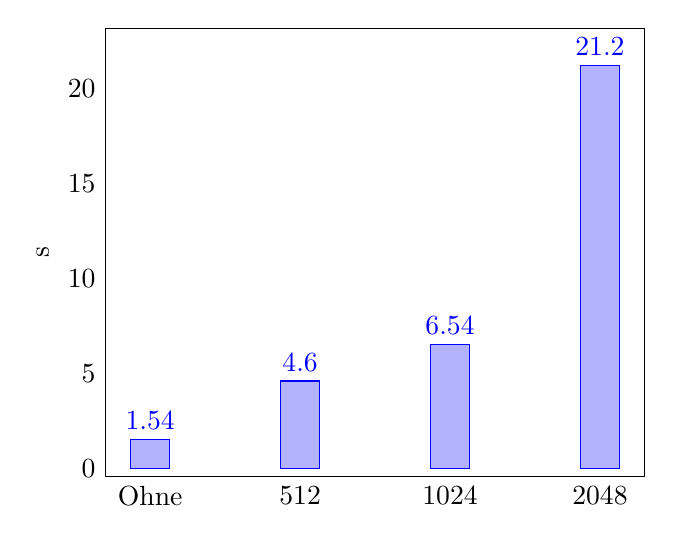
\begin{tikzpicture}
      \begin{axis}[%title  = ,
        ybar,
        bar width=.5cm,
        ylabel={s},
        %y axis line style = { opacity = 0 },
        %axis x line       = none,
        tickwidth         = 0pt,
        symbolic x coords = {Ohne, 512, 1024, 2048},
        xtick=data,
        nodes near coords,
      ]
      \addplot coordinates { 
        (Ohne, 1.54)
        (512, 4.60)
        (1024, 6.54)
        (2048, 21.20) 
      };
      \end{axis}
    \end{tikzpicture}
    \caption{Dauer der Bearbeitung von 100 Lognachrichten in Sekunden.}
    \label{fig:eval_barchart}
\end{figure}

Abbildung \ref{fig:eval_piecharts} zeigt zusätzlich die Zeitanteile, die im für die Pseudonymisierung zuständigen Plugin des Log-Proxy gemessen wurden, wie sie die jeweiligen Teilfunktionen bei den unterschiedlichen Schlüssellängen benötigten:
\begin{itemize}
  \item \textbf{MAC} -- Zeitanteil für die Berechnung des MACs, der für die Suche nach existierenden Pseudonymen genutzt wird, %(siehe Abschnitt \ref{sec_state_se_mac})
  \item \textbf{Schwellwert} -- Zeitanteil für die Verschlüsselung durch das kryptographische Schwellwertschema, %(siehe Abschnitt \ref{sec_impl_threshold})
  \item \textbf{Pseudonym} -- Zeitanteil für die Kommunikation mit dem Pseudonym-Service und die dort stattfindende Suche nach existierenden Pseudonymen.
\end{itemize} 

\begin{figure}[]
    \centering
    \begin{tikzpicture}
    %512
    \pie[
       rotate = 90, 
       radius = 2,
       color = {white, red!40, gray!40},
       %text = legend,
       after number={},
     ] {
         1/,
         2/,
         97/
     }
    
    %1024
     \pie[
        pos={4.5,0},
        rotate = 90, 
        radius = 2,
        color = {white, red!40, gray!40},
        %text = legend,
        after number={},
     ] {
         1/,
         6/,
         93/
     }
    %2048
     \pie[
         pos={9,0},
          rotate = 90, 
          radius = 2,
          color = {white, red!40, gray!40},
          text = legend,
          after number={},
      ] {
          1/MAC,
          36/Schwellwert, 
          63/Pseudonym     
      }
    \end{tikzpicture}
    \caption{Zeitlicher Anteil der verschiedenen Berechnungen im Pseudonymisierungs-Plugin bei  Schlüssellängen von 512 Bit (links), 1024 Bit (Mitte) und 2048 Bit (rechts).}
    \label{fig:eval_piecharts}
\end{figure}

Aus diesen Messungen ergibt sich, dass der größte Anteil an Bearbeitungszeit einer Lognachricht in der Abfrage des Pseudonym-Service nach einem existierenden Pseudonym und der Kommunikation zwischen dem Log-Proxy und dem Pseudonym-Service liegt.\\
Sollte sich die benötigte Zeit für die Bearbeitung von Logdaten im produktiven Einsatz als zu lang herausstellen, könnten die Komponenten zusammengeführt werden -- unter Verzicht auf die in Abschnitt \ref{sec_over_architecture} beschriebenen Vorteile bezogen auf die Sicherheit des Pseudonymzusammenhangs durch ein verteiltes System.\\
Mit steigenden Schlüssellängen steigt jedoch auch der Zeitanteil, den die Berechnungen des kryptographischen Schwellwertschemas benötigen, erheblich. Die Veränderung ist hier alleinig auf den asymmetrischen Teil des umgesetzten hybriden Schemas (siehe Abschnitt \ref{sec_impl_threshold_hybrid}) zurückzuführen, da sich der symmetrische Teil nicht verändert. Um die Performanz der Verschlüsselungsfunktion zu erhöhen, bietet sich die Nutzung von \textit{Elliptic Curve Cryptography} an (siehe Abschnitt \ref{sec_state_threshold_ecc}). Eine zusätzliche Möglichkeit ist auch die Implementierung dieser zeitkritischen Funktion durch eine maschinennähere Sprache als Python (wie beispielsweise C). 

Für die Berechnung der partiellen Entschlüsselungen und der kompletten Entschlüsselung eines Schlüsseltextes (und damit für die Aufdeckung eines Pseudonyms) wurde auf Performanzmessungen verzichtet. Diese Aktionen sind im umgesetzten System nicht zeitkritisch. Zusätzlich werden sie nur in seltenen Fällen -- nämlich bei der Aufdeckung eines Pseudonyms -- eingesetzt.

Insgesamt kam es bei den Messungen zu einigen Problemen, insbesondere wenn die Nachrichtenlast und damit die Rechenlast stieg:
\begin{itemize}
\item seltene Komplettausfälle des Systems aufgrund des Datenbanktreibers für die verwendete PostgreSQL-Datenbank,
\item Nicht-Behandlung von Nachrichten durch das unzuverlässige UDP-Protokoll.
\end{itemize}
Bessere (Mess-)Ergebnisse sollte das Deployment der Komponenten auf dafür ausgelegter Infrastruktur mit Standardlösungen für Python (Apache mit mod\_wsgi, uWSGI, ...) und entsprechender Rechenleistung bringen. Ebenso sollte die Nutzung von TCP-Verbindungen für das verwendete syslog-Protokoll mehr Zuverlässigkeit gewährleisten.\footnote{
  RFC 3195 (Reliable Delivery for syslog) beschreibt diese Erweiterung. Ob dies in der Praxis durch verbreitete Logdaten produzierende Geräte genutzt wird, bedarf allerdings weiterer Recherche.
}
